\section{Covariate-level Topic Analysis}

We now proceed to analyze the relationship between metadata information (i.e., document-level covariates) and topic proportions. We specify topical prevalence as 
\begin{align}
\mu_{d,k} = x_d^T \gamma_k= \text{party}_{d,k} + \text{state}_{d,k} + f_k(\text{t}_d) + g_k(\text{struct}_d), \label{prevalence}
\end{align} 
for all documents $d = 1,\dots,D$, and all topics $k = 1,\dots,K$, where 
\begin{align*}
g_k(\text{struct}_d) = g_{k}^{(1)}(\text{GDP}_d)+g_{k}^{(2)}(\text{unemployment}_d)+g_{k}^{(3)}(\text{immigrants}_d)+g_{k}^{(4)}(\text{votes}_d). 
\end{align*} 
That is, the political party and federal state of the respective parliamentarian associated with a document are specified as simple categorial dummy effects, while date and electoral-district structural covariates (GDP per capita, unemployment rate, percentage of immigrants, and the 2017 vote share) are modeled as additive smooth functions.

Note that approximate inference implies replacing $\mu_{d,k}$ with $\lambda_{d,k}$, i.e., with the mean of the approximate Gaussian posterior $q(\eta_{d,k})$. The estimates of $\Gamma = [\gamma_1 | \dots | \gamma_K]$ are updated in a Bayesian linear regression during each iteration of the EM algorithm in the M-step; for details see \cite{roberts2013structural}, p.\ 993.

While topical prevalence has an effect on the estimated topic proportions, the exact specification of topical prevalence is not a decisive factor. Both estimated topic proportions as well as heldout likelihood are in general only marginally affected by the concrete choice of the functional form. However, completely removing topical prevalence, in which case the model reduces to a CTM, does result in different topic proportions, as we show in section XXX. Since evaluation metrics such as heldout likelihood are mostly unaffected by the exact choice of topical prevalence and because the computational cost of fitting an stm is rather high, automatic model selection methods w.r.t.\ topical prevalence are not available. A reasonable specification of topical prevalence therefore relies on the domain knowledge of the researcher.

There exist different approaches to study the relationship between topic proportions and prevalence covariates. One possibility is to directly assess the maximum-a-posteriori (MAP) estimates $\hat{\Gamma}$ and $\hat{\Sigma}$, which are generated by the stm. Since the document-level topic proportions $\theta_d$ follow a logistic normal distribution (with mean $\mu_d$ and covariance matrix $\Sigma$), interpretation of the results can be difficult, since the logistic normal distribution is not very accessible. Nonetheless, we can visualize the relationship between a topic and a prevalence covariate, fixing other covariates at their median (or, for categorial variables, at the majority vote).

Alternatively, the estimated topic proportions can be used as the dependent variable of a new regression on prevalence covariates. However, in contrast to a standard regression setting, in this case the dependent variable has been estimated itself, before the regression is performed. Instead of simply using the MAP estimates of $\theta_d$ as the dependent variable, having access to the posterior distribution of the topic proportions, we can take account for the uncertainty of the dependent variable. This can be achieved by employing a sampling procedure known as the method of composition in the social sciences; see \cite{tanner2012tools}, p.52. This procedure is implemented in the \textit{stm} package through its function \textit{estimateEffect}.

In the following, we will first introduce the method of composition. We will discuss its implementation in the \textit{stm} package and provide alternative regression approaches based on the method of composition. Subsequently, we will evaluate the relationship between prevalence covariates and topic proportions by directly assessing the MAP estimates $\hat{\Gamma}$ and $\hat{\Sigma}$, as outlined above, and compare the results of both approaches.

\subsection{Method of Composition}

Let $\theta_{(k)}:=(\theta_{1,k}, \dots, \theta_{D,k}) \in [0,1]^{D}$ denote the proportions of the $k$-th topic for all $D$ documents. As stated, we want to perform a regression of these topic proportions $\theta_{(k)}$ on a subset $\tilde{X} \in \mathbb{R}^{D \times \tilde{P}}$ of prevalence covariates $X$. The true topic proportions are unknown, but the stm produces an estimate of the approximate posterior of $\theta_{(k)}$. A na{\"\i}ve approach would be to regress the estimated mode of the approximate posterior distribution on $\tilde{X}$. However, this approach neglects much of the information contained in the distribution. 

Instead, repeatedly sampling $\theta_{(k)}^*$ from the approximate posterior distribution, performing a regression for each sampled $\theta_{(k)}^*$ on $\tilde{X}$, and then sampling from the estimated distribution of 
icients, provides an i.i.d.\ sample from the marginal posterior distribution of regression coefficients. 

Sampling $\theta_{(k)}^*$ is achieved by first sampling the unnormalized topic proportions $\eta^*$ from the approximate posterior $q(\eta)$, applying the softmax $\theta^* = \text{softmax}(\eta^*)$ (element-wise, i.e., for each of the K-dimensional vectors of topic proportions), and lastly selecting the $k$-th column of $\theta^*$. Precisely, $q(\eta) = \prod_d q(\eta_d)$ is a normal distribution, which emerges from the laplace approximation within the variational inference scheme; for details see \cite{roberts2016model}, pp.\ 992-993. For clarity, we denote the approximate posterior of topic proportions as $q(\theta_{(k)} | X, W)$, in order to emphasize that the parameters of this distribution are learned from the observed data, i.e.\ prevalence covariates and words (note that we have no content variables included). Furthermore, let $\xi$ denote the regression coefficients from a regression of $\theta_{(k)}$ on $\tilde{X}$, and let $q(\xi| \tilde{X}, \theta_{(k)})$ be the approximate posterior distribution of these coefficients, i.e.\ given design matrix $\tilde{X}$ and response $\theta_{(k)}$.

The method of composition can now be described by repeating the following process $m$ times:
\begin{enumerate}
\item Draw $\theta_{(k)}^* \sim q(\theta_{(k)} | X, W)$.
\item Draw $\xi^* \sim q(\xi | \tilde{X}, \theta_{(k)})$.
\end{enumerate}
It then holds that $\xi_1^*, \dots, \xi_m^*$ is an i.i.d.\ sample from the marginal posterior
\begin{align*}
q(\xi | X, W) := \int_{\theta_{(k)}} q(\xi| \tilde{X}, \theta_{(k)}) q(\theta_{(k)} | X, W) \text{d} \theta_{(k)} = \int_{\theta_{(k)}} q(\xi, \theta_{(k)} | X, W) \text{d} \theta_{(k)}, 
\end{align*}
where $q(\xi, \theta_{(k)} | X, W) := q(\xi| \tilde{X}, \theta_{(k)}) q(\theta_{(k)} | X, W)$. Thus, by integrating over $\theta_{(k)}$, this approach allows incorporating information contained in the posterior distribution of $\theta_{(k)}$ when determining $\xi$.

\subsubsection{Implementation in the \textit{stm} package}

The R package \textit{stm} implements a simple OLS regression through its \textit{estimateEffect} function. However, this approach ignores that the sampled topic proportions are restricted to $(0,1)$. As expected, using this framework we frequently observe predicted proportions outside of $(0,1)$. Moreover, credible intervals are non-informative, due to violated model assumptions. 

\begin{figure}[h!]
  \centering
  \captionsetup{justification=centering,margin=2cm}
  \begin{subfigure}[b]{0.4\linewidth}
    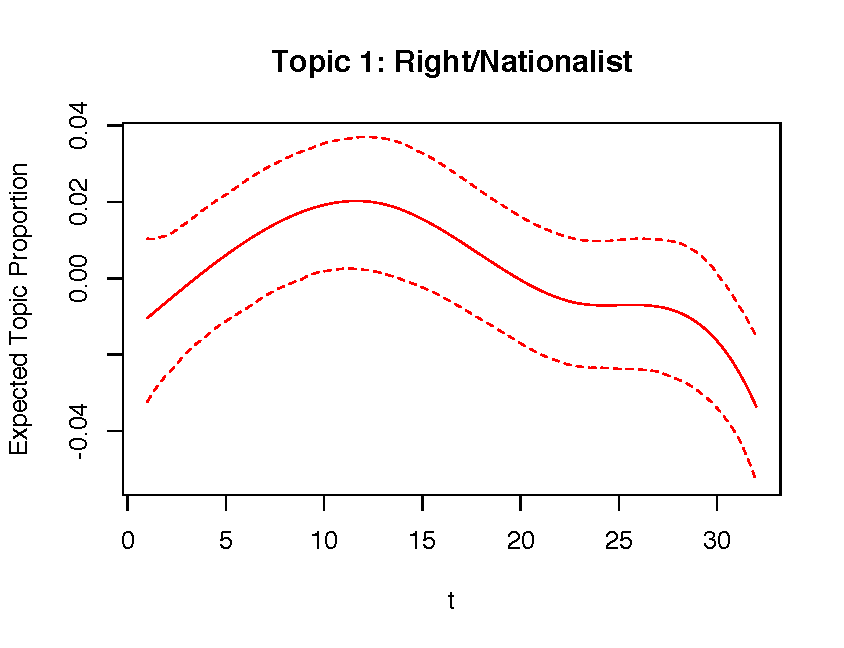
\includegraphics[width=\linewidth]{../plots/4_4/estEffect_topic1.pdf}
  \end{subfigure}
  \begin{subfigure}[b]{0.4\linewidth}
    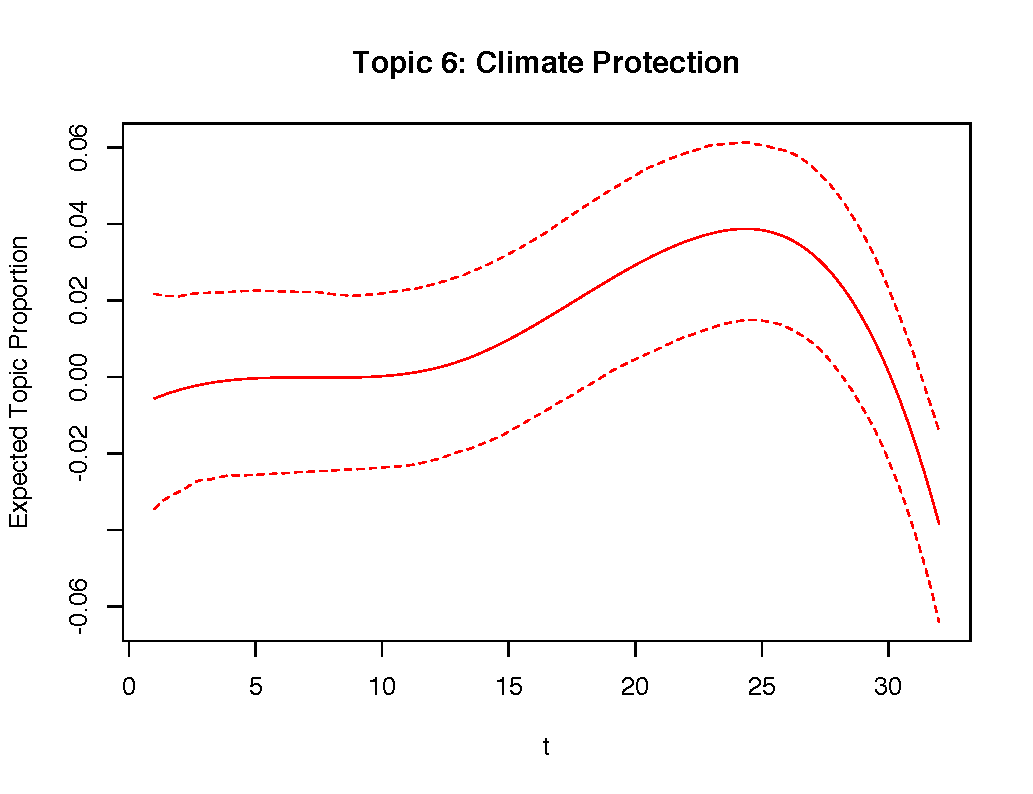
\includegraphics[width=\linewidth]{../plots/4_4/estEffect_topic6.pdf}
  \end{subfigure}
  \caption{Estimated prevalence of topics 1 and 6 over time, generated using \textit{estimateEffect} from the \textit{stm} package}
  \label{fig:coffee}
\end{figure}

\subsubsection{Alternative implementation}

We can attempt to improve the approach employed within the \textit{stm} package by replacing the OLS regression with a regression model that assumes a dependent variable in the interval $(0,1)$. However, note that since topic proportions are modeled separately, regardless of the specific model implied, distributional assumptions about $\theta_{(k)}$ will be violated. This is due to the fact that the the distribution of a subvector - and thus particularly of a single component - of $\theta_d$ is not of a simple form, when $\theta_d$ follows a logistic normal distribution, see e.g.\ \cite{atchison1980logistic}.

As shown by \cite{atchison1980logistic}, a distribution that can be used to approximate a logistic normal distribution is the Dirichlet distribution. However, note that the Dirichlet distribution assumes less interdependence among components than implied by the logistic normal distribution. In case of the Dirichlet distribution the univariate marginal distributions are beta. One possibility is thus to perform a separate beta regression for each topic proportion on $\tilde{X}$. 

As an alternative approximation we can employ a quasibinomial generalized linear model (GLM). Topic proportions can be rescaled and discretized and topics comprehended as classes, such that each rescaled topic proportion can be interpreted as the "number of successes" for the respective class. To match the underlying logistic normal distribution more closely, the quasi-likelihood furthermore allows for a flexible variance specification.

Note that $q(\xi| \theta_{(k)}, \tilde{X})$ is asymptotically normal for both the beta regression, see \cite{ferrari2004beta}, p.\ 17, and the quasibinomial GLM, see e.g.\ \cite{fahrmeir2007regression}, p. 285. Furthermore, in both cases we use a logit-link.

\subsubsection{Visualization}

We now apply the method of composition, based on either a beta regression or a quasibinomial GLM, in order to visualize covariate effects. Here we only visualize the results obtained by the quasibinomial GLM; the results of the beta regression, which show similar trends, are found in the appendix. Setting the number of simulations to 100, we sample $\xi^*_1, \dots, \xi^*_{100}$ from the  marginal posterior distribution $q(\xi | X, W)$. As mentioned, when visualizing the impact of a particular covariate, all other covariates are held at their median (or majority vote, if categorial), in line with the methodology employed in the \textit{stm} package.
Let $\tilde{X}^*$ denote the subset of $X$ where, apart from the variable of interest, each selected column consists of the median of the respective column of $X$. In order to plot the predicted effects, we then input $\tilde{X^*}\xi^*$ into the sigmoid function, which is the response function corresponding to a regression with logit-link, and calculate the predicted proportions. 

We exemplarily illustrate the relationship between covariates and topic proportions for topic 4 ("Social/Housing") and topic 6 ("Climate Protection"). The linear predictor of our regressions takes the same form as in  \eqref{prevalence}, i.e., we do not use a subset $\tilde{X}$, but the full set of prevalence covariates $X$, in order to estimate the effects, although we do not display each covariate included. For smooth effects, it is important to recall that their borders are inherently unstable, which is why one should refrain from (over-)interpreting them. For both continuous and categorical variables, black lines indicate the mean, and the shaded area represents 95\% credible intervals.

\begin{figure}[h!]
  \centering
  \captionsetup{justification=centering,margin=2cm}
  \begin{subfigure}[b]{0.49\linewidth}
    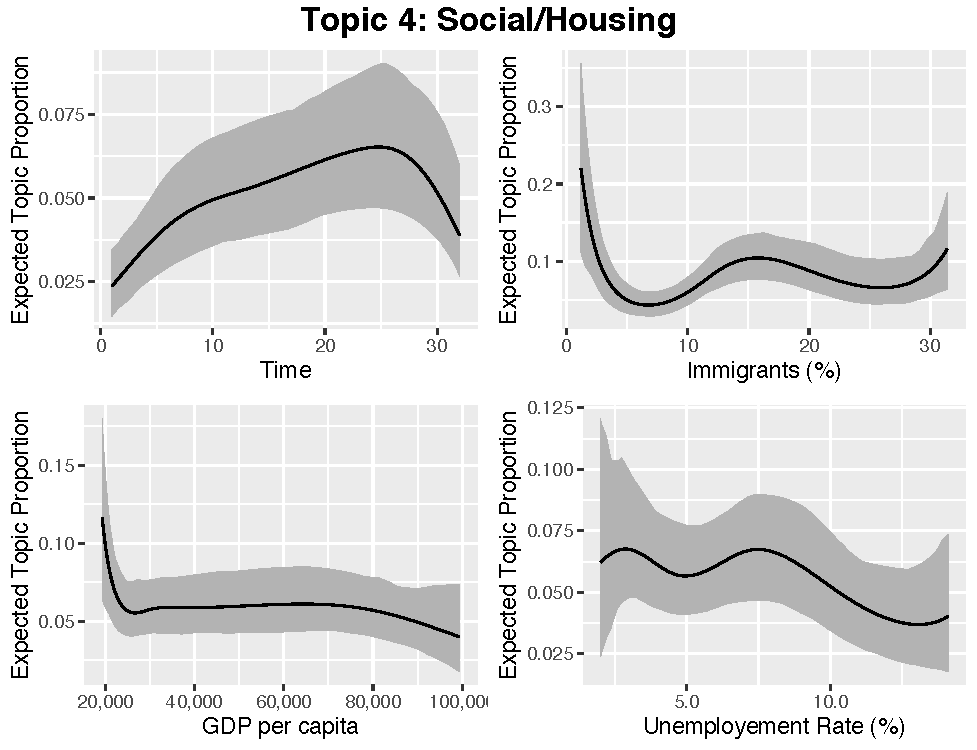
\includegraphics[width=\linewidth]{../plots/4_4/quasi_t4_cont.pdf}
  \end{subfigure}
  \begin{subfigure}[b]{0.49\linewidth}
    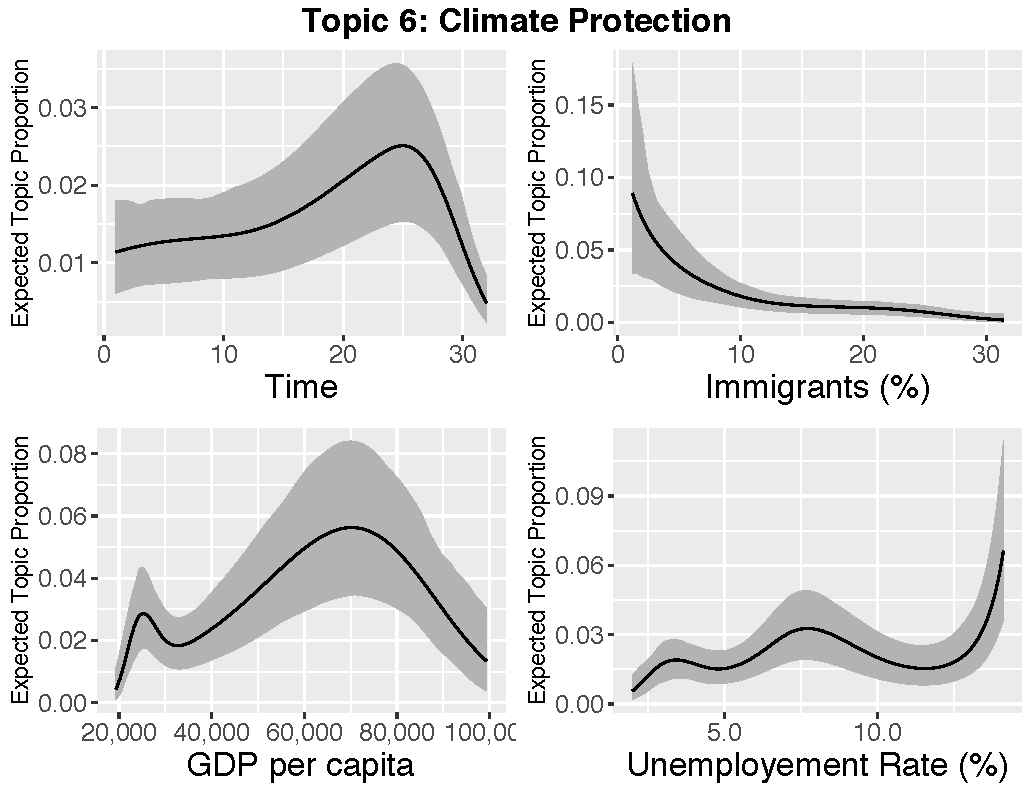
\includegraphics[width=\linewidth]{../plots/4_4/quasi_t6_cont.pdf}
  \end{subfigure}
  \caption{Mean and 95\% credible intervals for smooth effects, obtained using a quasibinomial GLM.}
  \label{fig:coffee}
\end{figure}

\begin{figure}[h!]
  \centering
  \captionsetup{justification=centering,margin=2cm}
  \begin{subfigure}[b]{0.49\linewidth}
    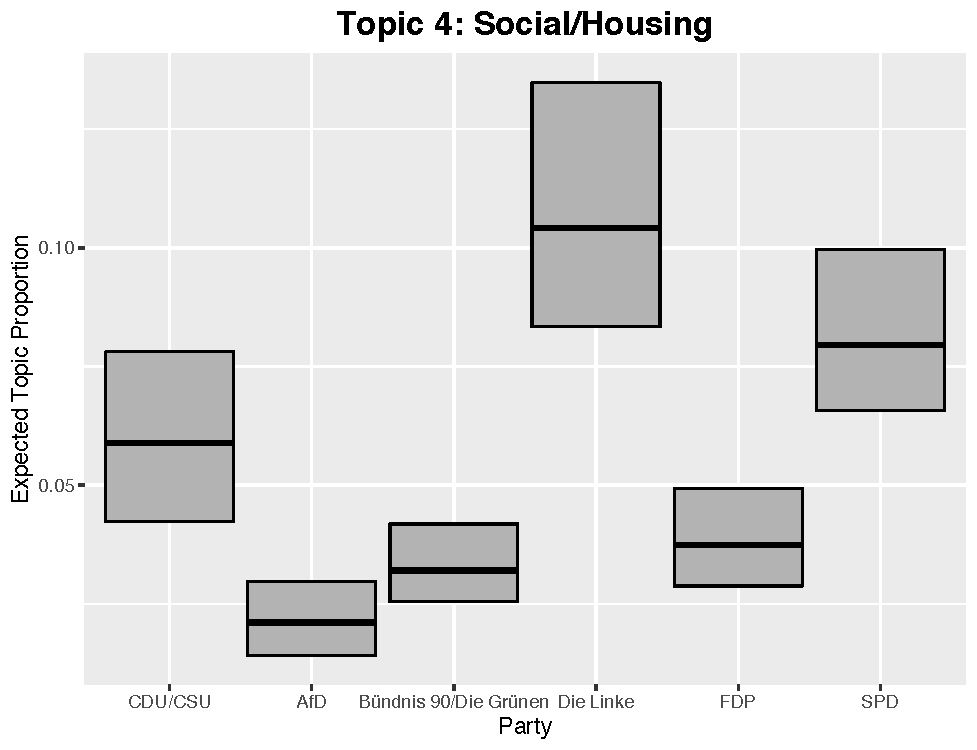
\includegraphics[width=\linewidth]{../plots/4_4/quasi_t4_cat.pdf}
  \end{subfigure}
  \begin{subfigure}[b]{0.49\linewidth}
    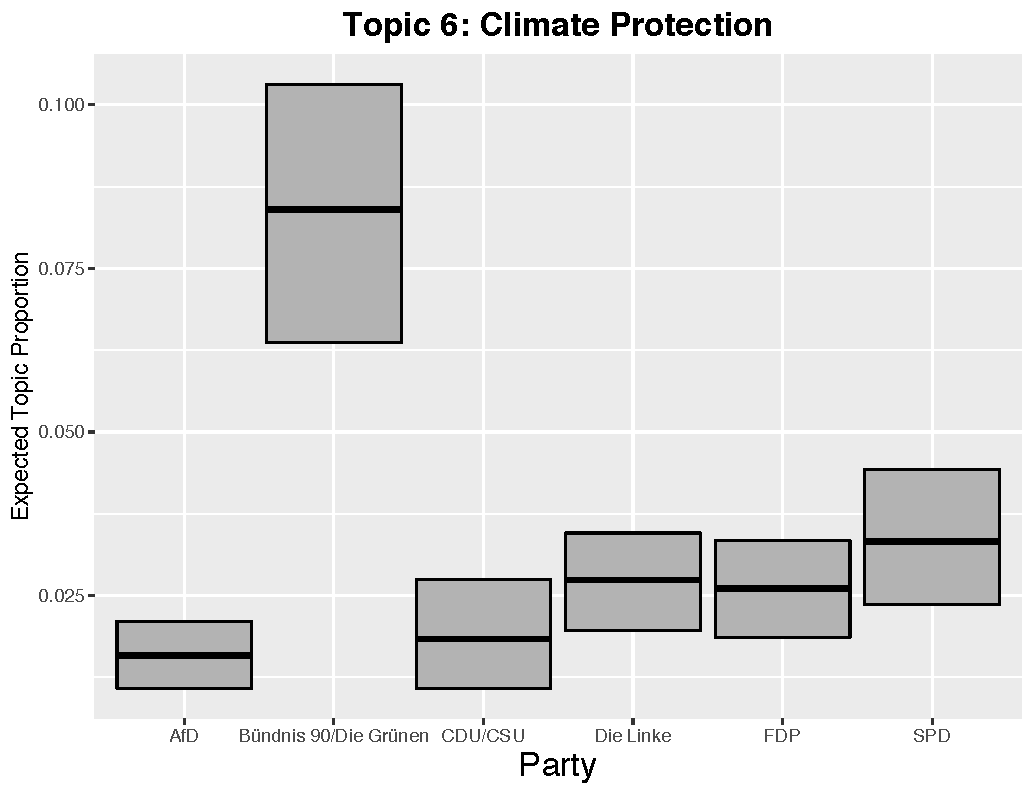
\includegraphics[width=\linewidth]{../plots/4_4/quasi_t6_cat.pdf}
  \end{subfigure}
  \caption{Mean and 95\% credible intervals for different political parties, obtained using a quasibinomial GLM.}
  \label{fig:coffee}
\end{figure}

For topic 4, "Social/Housing", we observe that most continuous variables have a small effect in absolute terms: the absolute variation in topic proportion across the covariate domains merely amounts to 4\%, compared to 8\% for topic 6. For most covariates the trend is rather ambiguous. Somewhat surprisingly, a very high unemployment rate is negatively linked to topic 4.

The effect of the political party on the relevance assigned to the topic "Social/Housing" is very much in line with a priori expectations: the left party and social democrats have the highest topical prevalence (15\% and 10\%, respectively), and the nationalist party the lowest (2\%).

For the smooth effects of topic 6, we observe its prevalence peaks in September 2019, corresponding to month t=25, decreasing afterwards. The absolute changes in topic proportions over time are rather small (around 3\%). The percentage of immigrants within an electoral district shows a negative relation to topic 6. Furthermore, topic 6 tends to be discussed more frequently in mid-income electoral districts than in high- and low-income districts. Finally, the link to the unemployment rate is somewhat ambiguous, although generally rather positive.

Regarding the relationship between the political party and the prevalence of topic "Climate Protection", as to be expected, we find high topical prevalence for the green party. Similar to the smooth effects, total variation in topic proportions across parties amounts to approximately 8\%.

Finally, the graph below shows a summary comparison of topical prevalence across all parties, for topics "Right/Nationalist", "Climate Protection" and "Social/Housing". The results are generally consistent with expectations. The proportions of topics "Climate Protection" and "Social/Housing" vary between 2\% and 9\% and between 2\% and 15\%, respectively. For topic 1, "Right/Nationalist", note how topical prevalence for the AfD party amounts to more than 40\%, implying that more than 40\% of the total content tweeted by AfD party members is about right-wing/nationalist issues, particularly immigration; for all other parties, topic 1 is rather marginal below 3\%.

\begin{figure}[h!]
  \centering
  \captionsetup{justification=centering,margin=2cm}
  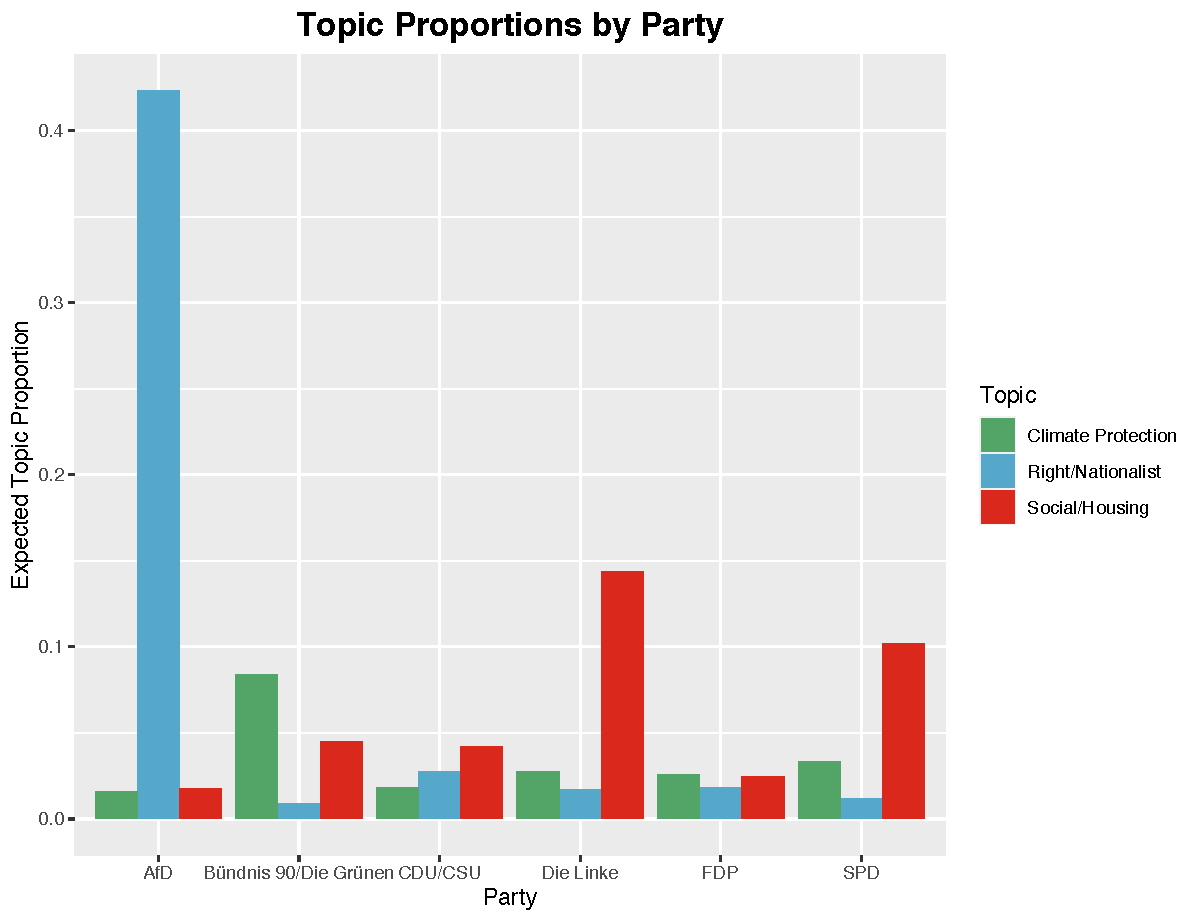
\includegraphics[scale = 0.5]{../plots/4_4/quasi_t146_cat.pdf}
  \caption{Topical prevalence by political party for topics 1, 4, and 6.}
  \label{fig:boat1}
\end{figure}

\subsection{Direct assessment using $\hat{\Gamma}$ and $\hat{\Sigma}$}

The \textit{stm} being an extension to the correlated topic model (\textit{CTM}), it is assumed that the topic proportions follow a logistic normal distribution, such that $\theta_d \sim \text{LogisticNormal}_{K-1}(\Gamma^Tx_d^T, \Sigma)$. Within the CTM, the Dirichlet distribution of the LDA has been replaced with a logistic normal distribution, in order to allow for a joint dependence among topics. Therefore, as mentioned above, separately modeling topic proportions is a simplification; in particular credible intervals should be treated with caution.

In order to examine the relation of prevalence covariates and topic proportions considering the joint dependence among the latter, we can attempt to directly use the output produced by the \textit{stm}: inference of the \textit{stm} involves finding the maximum-a-posteriori (MAP) estimate $\hat{\Gamma}$ and the maximum likelihood estimate $\hat{\Sigma}$. 

If we are interested in the question how a specific prevalence variable is related to topic proportions, similar to previous analyses, we can attempt to predict topic proportions based on a new design matrix $X^*$, where each column apart from the variable of interest corresponds to the median of the respective column of $X$. Ideally, in order to directly predict topic proportions, we would first draw a sample $\Gamma^*$ from the posterior distribution of $\Gamma$, and subsequently sample the topic proportions $\theta_d^*$ from a logistic normal with mean parameters $((\Gamma^*)^T (x_d^*)^T, \hat{\Sigma})$, where $\hat{\Sigma}$ is the maximum likelihood estimation of $\Sigma$. The resulting topic proportions would then correspond to a sample of the posterior predictive distribution of topic proportions. Unfortunately, the output of the stm does not allow for the possibility to draw a sample from the posterior distribution of $\Gamma$, but only provides its MAP estimate $\hat{\Gamma}$. 

Nevertheless, in order to get an impression how the assumed generative process of topic proportions in the stm behaves, we can plug in the estimates $\hat{\Gamma}$ and $\hat{\Sigma}$ into the logistic normal distribution and visualize sampled values from this distribution. Given a new observation $x_d^*$, we can sample $\theta_d^*$ from $\text{LogisticNormal}_{K-1}(\hat{\Gamma}^T(x_d^*)^T, \hat{\Sigma})$ by

\begin{enumerate}
\item Drawing $\eta_d^* \sim \mathcal{N}_{K-1}(\hat{\Gamma}^T(x_d^*)^T, \hat{\Sigma})$ and setting $\eta^*_{d,K} = 0$.
\item Mapping to the simplex, i.e., for all $k = 1,\dots,K$: $\theta_{d,k}^* = \frac{\exp(\eta^*_{d,k})}{\exp(\sum_{i=1}^{K} \eta^*_{d,i})}$.
\item Setting $\theta_d^* := (\theta_{d,1}^*, \dots \theta_{d,K}^*)^T$.
\end{enumerate}

We have repeated the above steps 1000 times for each input value of a selected variable, while fixing other variables at their median, and obtained the empirical mean as well as 95\% credible intervals. Plotting the results, we observe that while the mean shows a similar trend to our precious analyses, the obtained credible intervals are much broader.

\begin{figure}[h!]
    \centering
     \captionsetup{justification=centering,margin=2cm}
  \begin{subfigure}[b]{0.3\linewidth}
    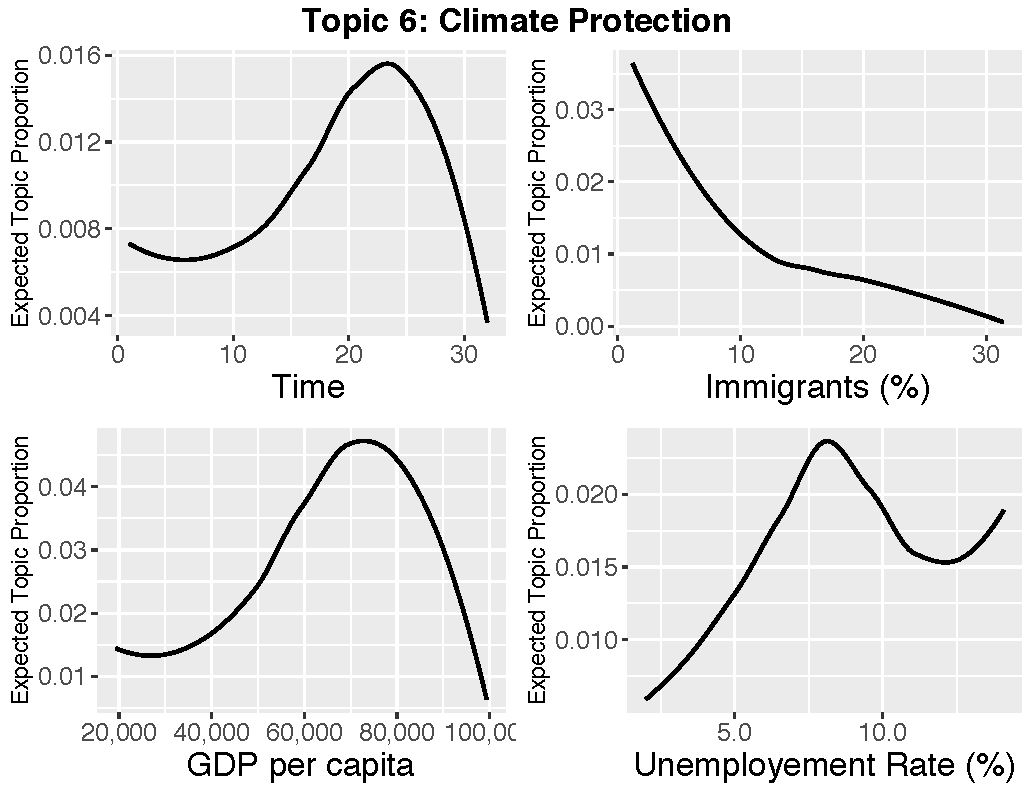
\includegraphics[width=\linewidth]{../plots/4_4/direct_t6_without_credible.pdf}
  \end{subfigure}
  \begin{subfigure}[b]{0.3\linewidth}
    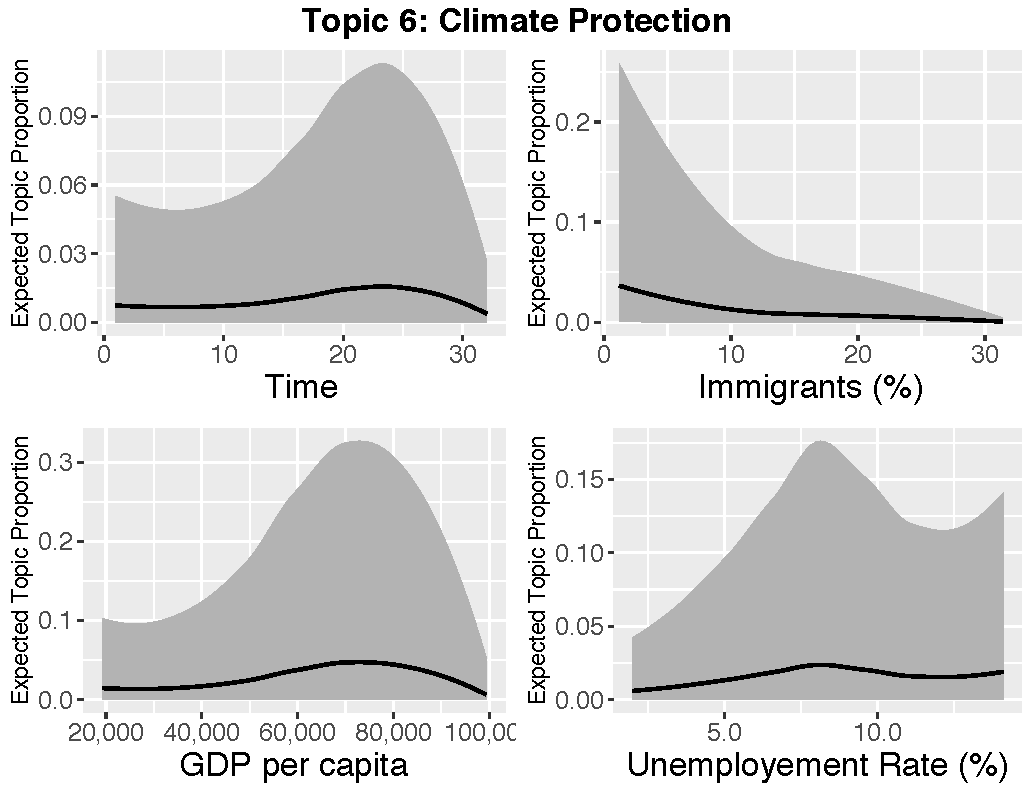
\includegraphics[width=\linewidth]{../plots/4_4/direct_t6_with_credible.pdf}
  \end{subfigure}
  \begin{subfigure}[b]{0.3\linewidth}
    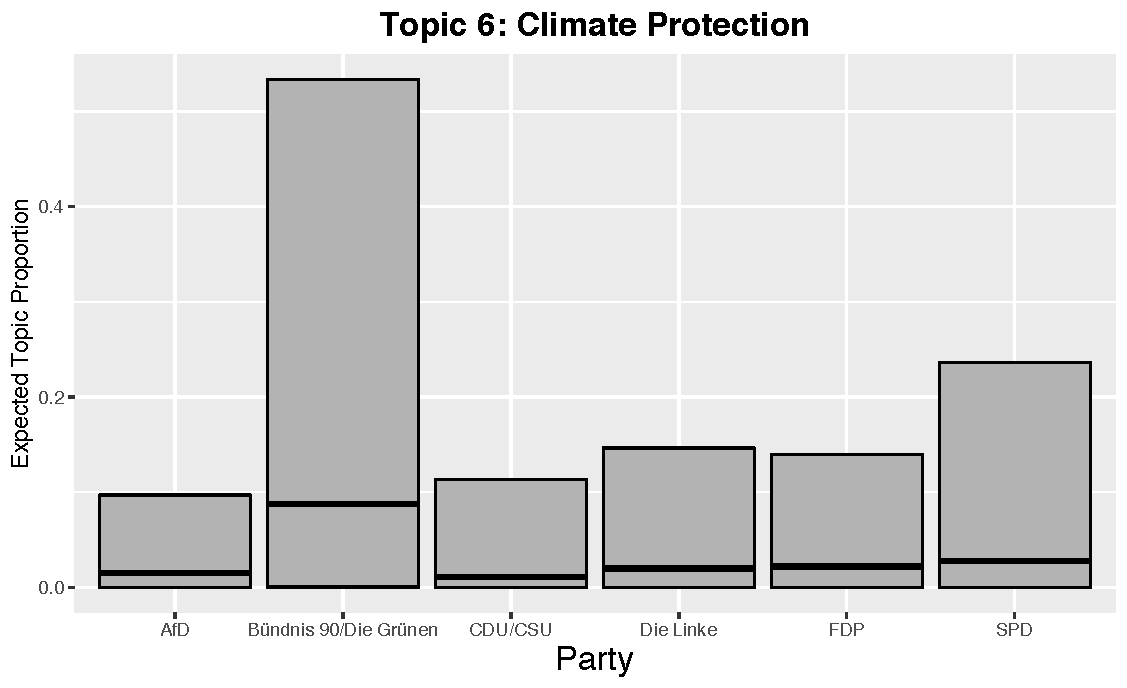
\includegraphics[width=\linewidth]{../plots/4_4/direct_t6_cat.pdf}
  \end{subfigure}
  \caption{Smooth effects without credible intervals, smooth effects with credible intervals and effect of the political party.}
  \label{fig:directassessment}
\end{figure}

The large fluctuations for a specific topic proportion can be ascribed to the fact that the unnormalized topic proportions are drawn from a $K-1$-dimensional \textit{multivariate} normal distribution, before the softmax is applied. Therefore, a single normalized proportion depends heavily on the sampled unnormalized proportions of the remaining topics. While the variance of a topic-specific unnormalized proportion is independent of the remaining unnormalized proportions and c.p.\ constant for an increasing number of topics, the application of the softmax function induces a large increase in the variance of a topic-specific normalized proportion.

We suspect that the magnitude of credible intervals in figure \ref{fig:directassessment} provides a more realistic picture than in case of a separate modeling of topic proportions, since the usage of the logistic normal distribution of topic proportions is an implicit assumption made within the stm that there is a dependence among topics, as argued above. This ultimately produces a large variance of the univariate marginal distributions of topic proportions, as can be observed. While ideally we should sample $\Gamma$ from its posterior distribution instead of plugging in its MAP estimate, our results suggest that there is a discrepancy between the assumed distribution of topic proportions in the generative process of the stm, and the impression we gain of the distribution of topic proportions from a separate modeling of topics within the method of composition.

